\chapter{Introduction}

The aim of this project is to run a complete tournament
of the Platypus game, which has been stated to be infeasible
by my supervisor James Harland in his lectures for the
Computing Theory course.
The Platypus game is related to the \emph{busy beaver} game,
which aims to find the Turing machine of a given complexity
which generates the longest string on a tape and eventually halts.
But the Platypus game is difficult to run for different reasons: it
involves a finite and cyclic board rather than an infinite tape, and
the length of a Platypus game can run is bounded, but the search space
is much larger due to the Platypus game involving two competing
machines sharing the board.

\section{The Platypus game}

The \emph{Platypus} game is is a theoretical game introduced in the
Computing Theory course in RMIT, used to teach automata
(particularly Turing machines) and complexity theory.
The Platypus game is played by two 4-state Turing machine
\emph{players}, which share a two-symbol board with 21 cells. The states
are named Kangaroo, Emu, Wombat and Platypus, and the symbols
are named Yellow and Green. (These names are sometimes shortened
to their initials for brevity.) One such machine is represented in three
different ways in Figure~\ref{fig:representations}. Note that a transition
% In unrelated conversation I hear "graphical representation" more, but
% I interpret it first as "visual" and then realise it means "using a graph".
is written in the graph representation as $S_1 \rightarrow S_2, D$ where
$S_1$ is the symbol read, $S_2$ the symbol written and $D$ the direction
to move in. The board is initially all Yellow.

All machines start in the Kangaroo state, and the game ends when
both players have made 50 moves each, or a player with a Platypus
state reads a Green cell.
Players earn points in a game by changing the colours of cells; the
winner has the most points.

\begin{figure}
  \begin{center}
    \begin{tabular}{rr|ccccccc}
      \hline
      From & Colour & Y & G & Y & G & Y & G & Y \\
      & Animal & K & K & E & E & W & W & P \\
      \hline
      To & Colour & G & Y & G & G & G & Y & G \\
      & Animal & W & K & W & E & E & E & K \\
      & Direction & G & G & G & G & W & G & G \\
      \hline
      \multicolumn{2}{r}{Hexadecimal} &
      \texttt{A} & \texttt{F} & \texttt{A} & \texttt{C} & \texttt{4} & \texttt{D} & \texttt{E}
    \end{tabular}
    
    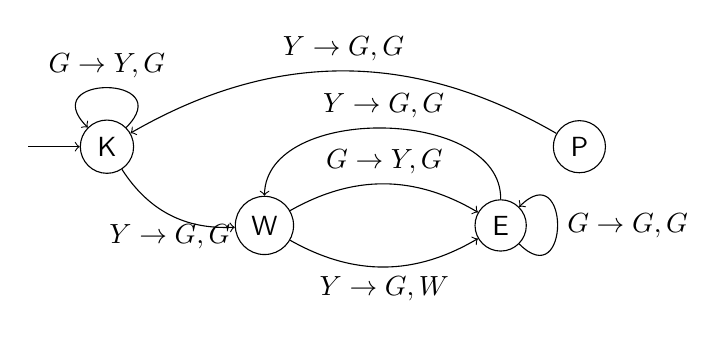
\begin{tikzpicture}
      \node[draw, circle] (P) at (6, 0) {\sffamily P};
      \node[draw, circle] (W) at (2, -1) {\sffamily W};
      \node[draw, circle] (E) at (5, -1) {\sffamily E};
      \node[draw, circle] (K) at (0, 0) {\sffamily K};
      \draw[->] (-1, 0) to (K);
      \draw[->] (P) to[bend right] node[midway, above] {$\q{Y} \rightarrow \q{G}, \q{G}$} (K);
      \draw[->] (W) to[bend left] node[midway, above] {$\q{G} \rightarrow \q{Y}, \q{G}$} (E);
      \draw[->] (W) to[bend right] node[midway, below] {$\q{Y} \rightarrow \q{G}, \q{W}$} (E);
      \draw[->] (E) to[in=45, out=-45, looseness=5] node[midway, right] {$\q{G} \rightarrow \q{G}, \q{G}$} (E);
      \draw[->] (E) to[bend right=90] node[midway, above] {$\q{Y} \rightarrow \q{G}, \q{G}$} (W);
      \draw[->] (K) to[in=135, out=45, looseness=5] node[midway, above] {$\q{G} \rightarrow \q{Y}, \q{G}$} (K);
      \draw[->] (K) to[bend right] node[midway, below] {$\q{Y} \rightarrow \q{G}, \q{G}$} (W);
    \end{tikzpicture}
  \end{center}
  \caption{A Platypus machine represented in three different ways.}
  \label{fig:representations}
\end{figure}

\section{The Platypus tournament}

A Platypus \emph{tournament} may be played, to find a machine
out of some set of machines which wins the most matches (or
earns the most points in total, if multiple machines win the
same largest number of matches). A tournament involves playing
every player against every player, including matches
with machines playing themselves and matches which have the
players reversed to other matches; a tournament of $n$ matches
thus involves playing $n^2$ matches%
\footnote{The Computing Theory course defines a match between
  machines $a$ and $b$ to be playing a Platypus game with players
  $a$ and $b$, and another game with players $b$ and $a$. This
  definition would have $\frac12 n(n-1)$ matches, as the outcome of
  a match does not depend on the order the machines. 
  It is however useful to separate the two times the game is played
  (and I analyse them separately in \autoref{chap:results}), so I
  define a match to be playing just one game, and the result of
  a match does depend on the order of the machines.}
The \emph{complete tournament} involves playing every possible
matches with every possible machine, of which there are $2^{56}$
(approximately 72 quadrillion) matches. If one could run 1 billion
Platypus matches per second, they would still need 2.3 years to
run every possible match.

It is interesting to compare the effort of running a complete
tournament to performing a brute-force attack on the insecure
\emph{Data Encryption Standard} (DES) encryption algorithm, which
has $2^{56}$ possible keys. The \emph{Deep Crack} machine built by the
Electronic Frontier Foundation used less than US\$250,000 of custom
hardware to search the entire key space in about nine days, testing
88 billion keys per second \cite{deep-crack}. A more recent system using
\emph{field-programmable gate arrays} can search 768 billion keys per
second, searching the entire key space in 26 hours \cite{crack.sh}. But the
Platypus game is not an encryption algorithm, so the amount of
effort can (more easily) be reduced by analysis of the Platypus game.
The result of a Platypus tournament contains more data than
which key correctly decrypts a message however, and Platypus matches
have variable lengths (whereas DES encryption takes constant time with
regards to the key), so parallelisation is more difficult.

Thus the project requires both high-level and low-level optimisations,
which I found very interesting. The number of matches can be
reduced by a factor $25\times$ by eliminating equivalent machines
(as in Chapter 2), and the remaining machines must be tested with
high throughput (for which I eventually settled on GPGPU with cloud
computing, as described in Chapter 3). I was then able to run the full
tournament in nine days.

\section{Representing Platypus machines}
\label{sec:representation}

A computer program requires a concrete representation of the abstract
concept of a Platypus machine, in order to use the machine.
There are some desirable properties of a representation:

\begin{itemize}
\item It should be easy to iterate all the possible Platypus machines.
\item Finding a transition by input to the transition function should be fast.%
\item The representation should be compact, to allow for fitting many
  machines in memory.
\end{itemize}

I represent a Platypus machine as an integer in the range
$[0, 2^{28})$. The 28 bits of a machine are divided between its seven
defined 4-bit transitions; each 4-bit transition is comprised of
1 bit for the symbol written by the player (Green or Yellow), 2 bits
for the state to transition to (Platypus, Wombat, Emu or Kangaroo),
and 1 bit for the direction that the player moves (towards the wattle
or the ghost gum).

The mapping between each abstract value used by the machine and
concrete values used by an implementation is ultimately arbitrary. I
use a mapping which allows using the indexes of the tabular format used
in the course material for Computing Theory, as presented in
Figure~\ref{fig:representations}. Green is represented as 0, and Yellow as 1;
and a Platypus is represented as 0, Wombat as 1, Emu as 2, and Kangaroo
as 3. The transition for reading a cell of colour $c$ with animal $a$
starts from the $4(2a + c - 1)$th bit (starting at 0). Note that the transition
for reading a Green cell as Platypus starts at the $-4$th bit as $a = 0$ and
$c = 0$, but we will never perform a transition in that situation.

The representation provides all the desired properties:

\begin{itemize}
\item All machines may be iterated over by producing successive
  integers, which is trivial.
\item A transition may be found by extracting a sequence of bits from
  the integer, which is very fast. The Common Lisp language \cite{common-lisp}
  provides the functions \texttt{ldb} (``load byte'') and
  \texttt{dpb} (``deposit byte'') for extracting and replacing sequences
  of bits from integers; I use these functions extensively in my implementation.
\item The representation is an \emph{implicit data structure}
  \cite{implicit-data-structures}, requiring the minimum necessary
  number of bits to encode a machine; Common Lisp implementations
  also do not perform heap allocations for small integers (``fixnums'').
\end{itemize}

Additionally, a machine using the representation may be efficiently
updated by replacing part of an integer; this update does not modify
the original machine, allowing for a functional programming style
while constructing and modifying machines while detecting
equivalences. This representation is implemented in the file
\texttt{Code/representation.lisp}.

\section{Conventions}

The real time taken to perform computations was measured on my
desktop, which has a 12-core/24-thread Ryzen 5900X processor with 16GB
of memory, and a RX 580 graphics card with 8GB of memory. I report
many durations in \emph{CPU-seconds} -- the sum of all times taken
by each core -- as many problems are run across all cores.

\section{Infrastructure}

The code and {\fontfamily{lmr}\selectfont \LaTeX} sources for this report
are hosted on GitHub at \url{https://github.com/no-defun-allowed/platypus-games-without-frontiers/}.
The code is predominantly written in Common Lisp, using some
extensions specific to the Steel Bank Common
Lisp\footnote{\url{http://sbcl.org/}} implementation. The GPGPU code is
written using Python, OpenCL and the PyOpenCL library.
I use cloud compute provided by the RMIT AWS Cloud Supercomputing
(RACE) Hub.